\chapter{Sorting Algorithms}
\chaplabel{sorting}

This chapter discusses algorithms for sorting a set of #n# items.
This might seem like a strange topic for a book on data structures, but
there are several good reasons for including it here.  The most obvious
reason is that two of these sorting algorithms (quicksort and heap-sort)
are intimately related to two of the data structures we have already
studied (random binary search trees and heaps, respectively).

The first part of this chapter discusses algorithms that sort using only
comparisons and presents three algorithms that run in $O(#n#\log #n#)$
time.  As it turns out, all three algorithms are asymptotically optimal;
no algorithm that uses only comparisons can avoid doing roughly $#n#\log
#n#$ comparisons in the worst case and even the average case.

Before continuing, we should note that any of the #SSet# or priority
#Queue# implementations presented in previous chapters can also
be used to obtain an $O(#n#\log #n#)$ time sorting algorithm.
For example, we can sort #n# items by performing #n# #add(x)#
operations followed by #n# #remove()# operations on a #BinaryHeap#
or #MeldableHeap#. Alternatively, we can use #n# #add(x)# operations
on any of the binary search tree data structures and then perform an
in-order traversal (\excref{tree-traversal}) to extract the elements in
sorted order.  However, in both cases we go through a lot of overhead to
build a structure that is never fully used.  Sorting is such an important
problem that it is worthwhile developing direct methods that are as fast,
simple, and space-efficient as possible.

The second part of this chapter shows that, if we allow other
operations besides comparisons, then all bets are off.  Indeed, by using
array-indexing, it is possible to sort a set of #n# integers in the range
$\{0,\ldots,#n#^c-1\}$ in $O(c#n#)$ time.



\section{Comparison-Based Sorting}

\index{comparison-based sorting}%
\index{sorting algorithm!comparison-based}%
In this section, we present three sorting algorithms: merge-sort,
quicksort, and heap-sort.  Each of these algorithms takes an input array #a#
and sorts the elements of #a# into non-decreasing order in $O(#n#\log #n#)$
(expected) time.  These algorithms are all \emph{comparison-based}.
\javaonly{Their second argument, #c#, is a #Comparator#
\index{Comparator@#Comparator#}%
that implements
the #compare(a,b)#
\index{compare@#compare(a,b)#}%
method.}  These algorithms don't care what type
of data is being sorted; the only operation they do on the data is
comparisons using the #compare(a,b)# method. Recall, from \secref{sset},
that #compare(a,b)# returns a negative value if $#a#<#b#$, a positive
value if $#a#>#b#$, and zero if $#a#=#b#$.

\subsection{Merge-Sort}
\seclabel{merge-sort}

\index{merge-sort}%
The \emph{merge-sort} algorithm is a classic example of recursive divide
and conquer: 
\index{divide-and-conquer}%
If the length of #a# is at most 1, then #a# is already
sorted, so we do nothing.  Otherwise, we split #a# into two halves,
$#a0#=#a[0]#,\ldots,#a[n/2-1]#$ and $#a1#=#a[n/2]#,\ldots,#a[n-1]#$.
We recursively sort #a0# and #a1#, and then we merge (the now sorted)
#a0# and #a1# to get our fully sorted array #a#:
\javaimport{ods/Algorithms.mergeSort(a,c)}
\cppimport{ods/Algorithms.mergeSort(a)}
\pcodeimport{ods/Algorithms.mergeSort(a)}
An example is shown in \figref{merge-sort}.
\begin{figure}
  \begin{center}
    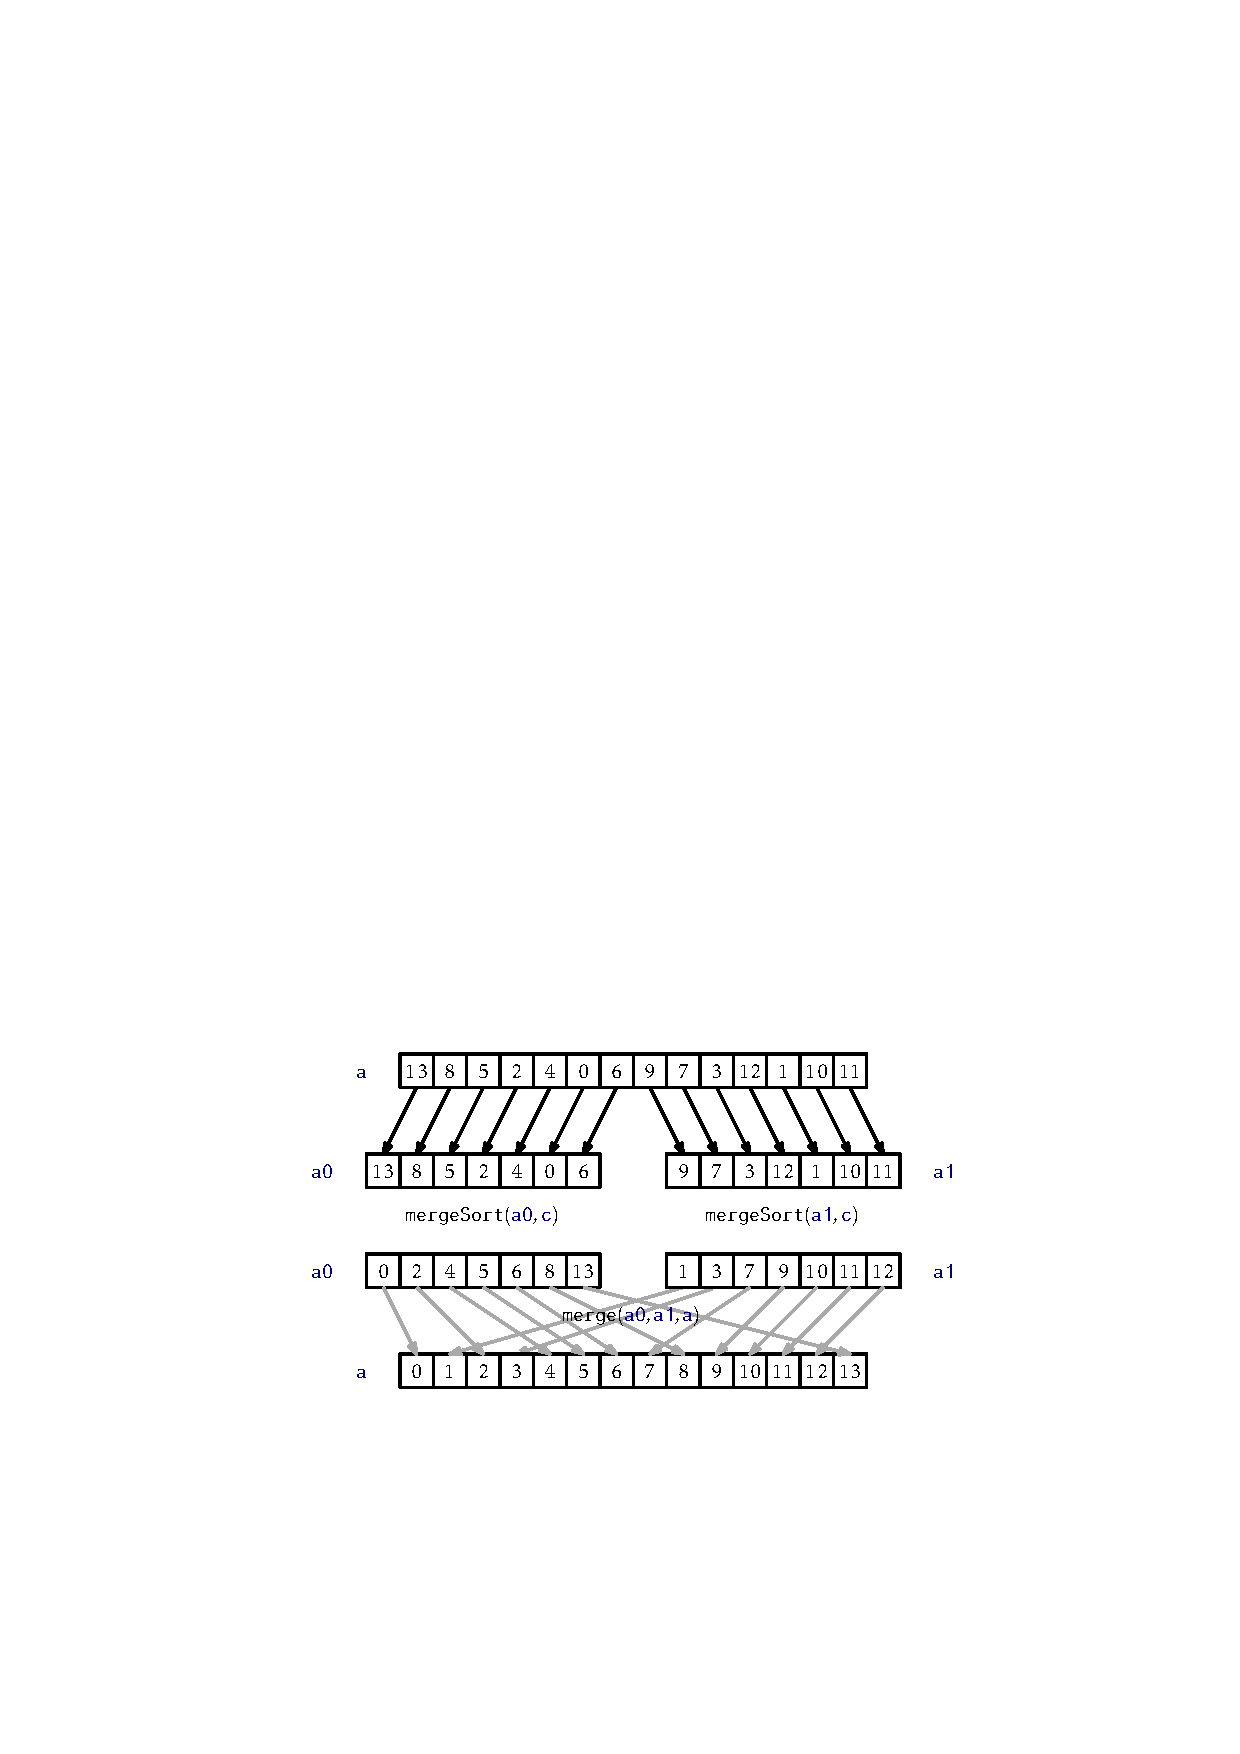
\includegraphics[width=\ScaleIfNeeded]{figs/mergesort}
  \end{center}
  \caption[Merge sort]{The execution of #mergeSort(a,c)#}
  \figlabel{merge-sort}
\end{figure}

Compared to sorting, merging the two sorted arrays #a0# and #a1# is
fairly easy.  We add elements to #a# one at a time.  If #a0# or #a1#
is empty, then we add the next elements from the other (non-empty)
array. Otherwise, we take the minimum of the next element in #a0# and
the next element in #a1# and add it to #a#:
\javaimport{ods/Algorithms.merge(a0,a1,a,c)}
\cppimport{ods/Algorithms.merge(a0,a1,a)}
\pcodeimport{ods/Algorithms.merge(a0,a1,a)}
Notice that the #merge(a0,a1,a,c)# algorithm performs at most $#n#-1$
comparisons before running out of elements in one of #a0# or #a1#.

To understand the running-time of merge-sort, it is easiest to think
of it in terms of its recursion tree.  Suppose for now that #n# is a
power of two, so that $#n#=2^{\log #n#}$, and $\log #n#$ is an integer.
Refer to \figref{mergesort-recursion}. Merge-sort turns the problem of
sorting #n# elements into two problems, each of sorting $#n#/2$ elements.
These two subproblem are then turned into two problems each, for a total
of four subproblems, each of size $#n#/4$. These four subproblems become eight
subproblems, each of size $#n#/8$, and so on.  At the bottom of this process,
$#n#/2$ subproblems, each of size two, are converted into #n# problems,
each of size one.  For each subproblem of size $#n#/2^{i}$, the time
spent merging and copying data is $O(#n#/2^i)$.  Since there are $2^i$
subproblems of size $#n#/2^i$, the total time spent working on problems
of size $2^i$, not counting recursive calls, is
\[
       2^i\times O(#n#/2^i) = O(#n#) \enspace .
\]
Therefore, the total amount of time taken by merge-sort is
\[
   \sum_{i=0}^{\log #n#} O(#n#) = O(#n#\log #n#) \enspace .
\]

\begin{figure}
  \begin{center}
    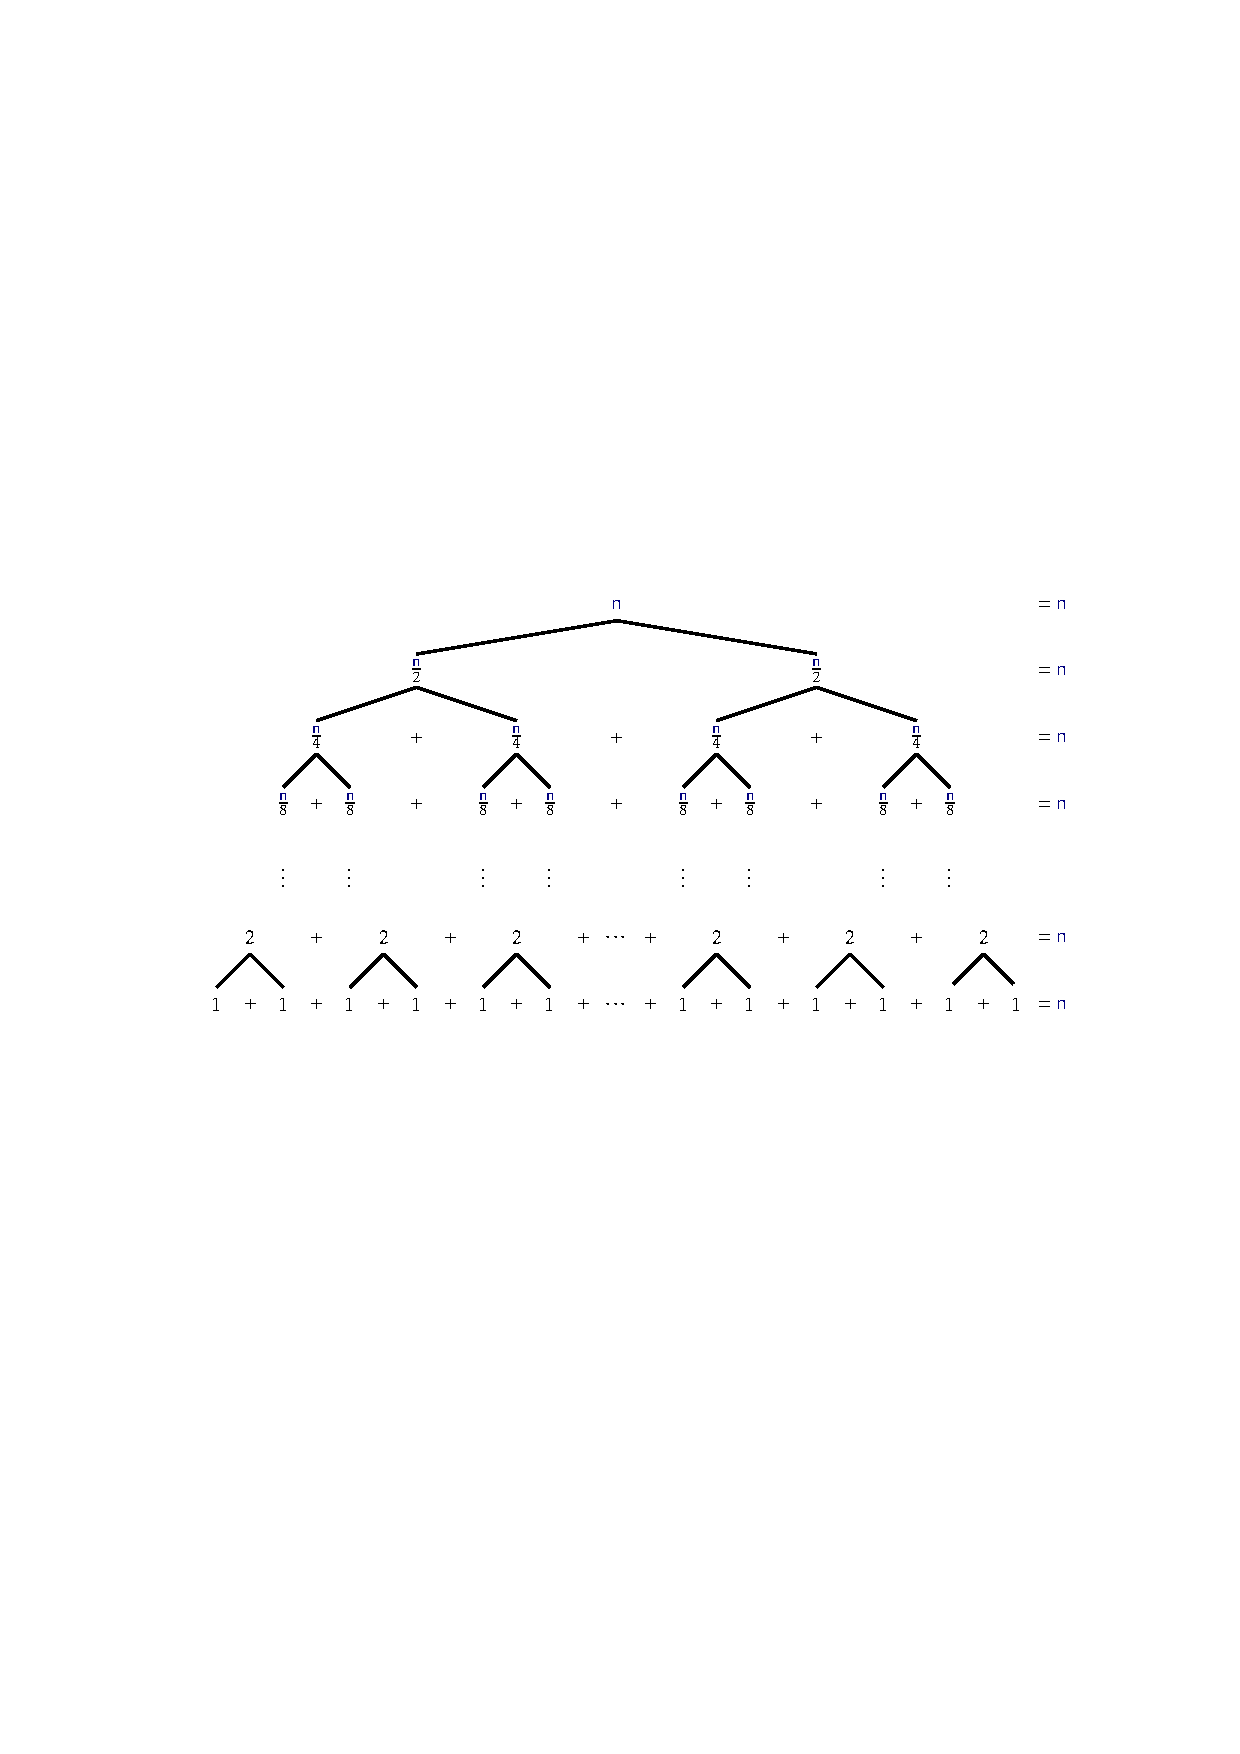
\includegraphics[width=\ScaleIfNeeded]{figs/mergesort-recursion}
    \caption{The merge-sort recursion tree.}
    \figlabel{mergesort-recursion}
  \end{center}
\end{figure}

The proof of the following theorem is based on preceding analysis,
but has to be a little more careful to deal with the cases where #n#
is not a power of 2.
\begin{thm}
  The \javaonly{#mergeSort(a,c)#}\cpponly{mergeSort(a)}\pcodeonly{merge\_sort(a)} algorithm runs in $O(#n#\log #n#)$ time and
  performs at most $#n#\log #n#$ comparisons.
\end{thm}

\begin{proof}
The proof is by induction on $#n#$.  The base case, in which $#n#=1$,
is trivial; when presented with an array of length 0 or 1 the algorithm
simply returns without performing any comparisons.

Merging two sorted lists of total length $#n#$ requires at most $#n#-1$
comparisons. Let $C(#n#)$ denote the maximum number of comparisons performed by
#mergeSort(a,c)# on an array #a# of length #n#.  If $#n#$ is even, then we apply the inductive hypothesis to
the two subproblems and obtain
\begin{align*}
  C(#n#) 
  &\le #n#-1 + 2C(#n#/2) \\
  &\le #n#-1 + 2((#n#/2)\log(#n#/2)) \\
  &= #n#-1 + #n#\log(#n#/2) \\
  &= #n#-1 + #n#\log #n#-#n# \\
  &< #n#\log #n# \enspace .
\end{align*}
The case where $#n#$ is odd is slightly more complicated.  For this case,
we use two inequalities that are easy to verify:
\begin{equation}
  \log(x+1) \le \log(x) + 1 \enspace , \eqlabel{log-ineq-a}
\end{equation}
for all $x\ge 1$ and
\begin{equation}
  \log(x+1/2) + \log(x-1/2) \le 2\log(x) \enspace , \eqlabel{log-ineq-b}
\end{equation}
for all $x\ge 1/2$.  Inequality~\myeqref{log-ineq-a} comes from the fact that $\log(x)+1 = \log(2x)$ while \myeqref{log-ineq-b} follows from the fact that $\log$ is a concave function.  With these tools in hand we have, for odd #n#,
\begin{align*}
  C(#n#) 
  &\le #n#-1 + C(\lceil #n#/2 \rceil) + C(\lfloor #n#/2 \rfloor) \\
  &\le #n#-1 + \lceil #n#/2 \rceil\log \lceil #n#/2 \rceil 
           + \lfloor #n#/2 \rfloor\log \lfloor #n#/2 \rfloor \\
  &= #n#-1 + (#n#/2 + 1/2)\log (#n#/2+1/2) 
           + (#n#/2 - 1/2) \log (#n#/2-1/2) \\
  &\le #n#-1 + #n#\log(#n#/2) + (1/2)(\log (#n#/2+1/2) 
           - \log (#n#/2-1/2)) \\
  &\le #n#-1 + #n#\log(#n#/2) + 1/2 \\
  &< #n# + #n#\log(#n#/2) \\
  &= #n# + #n#(\log#n#-1) \\
  &= #n#\log#n# \enspace . \qedhere
\end{align*} 
\end{proof}

\subsection{Quicksort}

\index{quicksort}%
The \emph{quicksort} algorithm is another classic divide and conquer
algorithm.  Unlike merge-sort, which does merging after solving the two
subproblems, quicksort does all of its work upfront.

Quicksort is simple to describe:  Pick a random \emph{pivot} element,
\index{pivot element}%
#x#, from #a#; partition #a# into the set of elements less than #x#, the
set of elements equal to #x#, and the set of elements greater than #x#;
and, finally, recursively sort the first and third sets in this partition.
An example is shown in \figref{quicksort}.
\javaimport{ods/Algorithms.quickSort(a,c).quickSort(a,i,n,c)}
\cppimport{ods/Algorithms.quickSort(a).quickSort(a,i,n)}
\pcodeimport{ods/Algorithms.quickSort(a).quickSort(a,i,n)}
\begin{figure}
  \begin{center}
    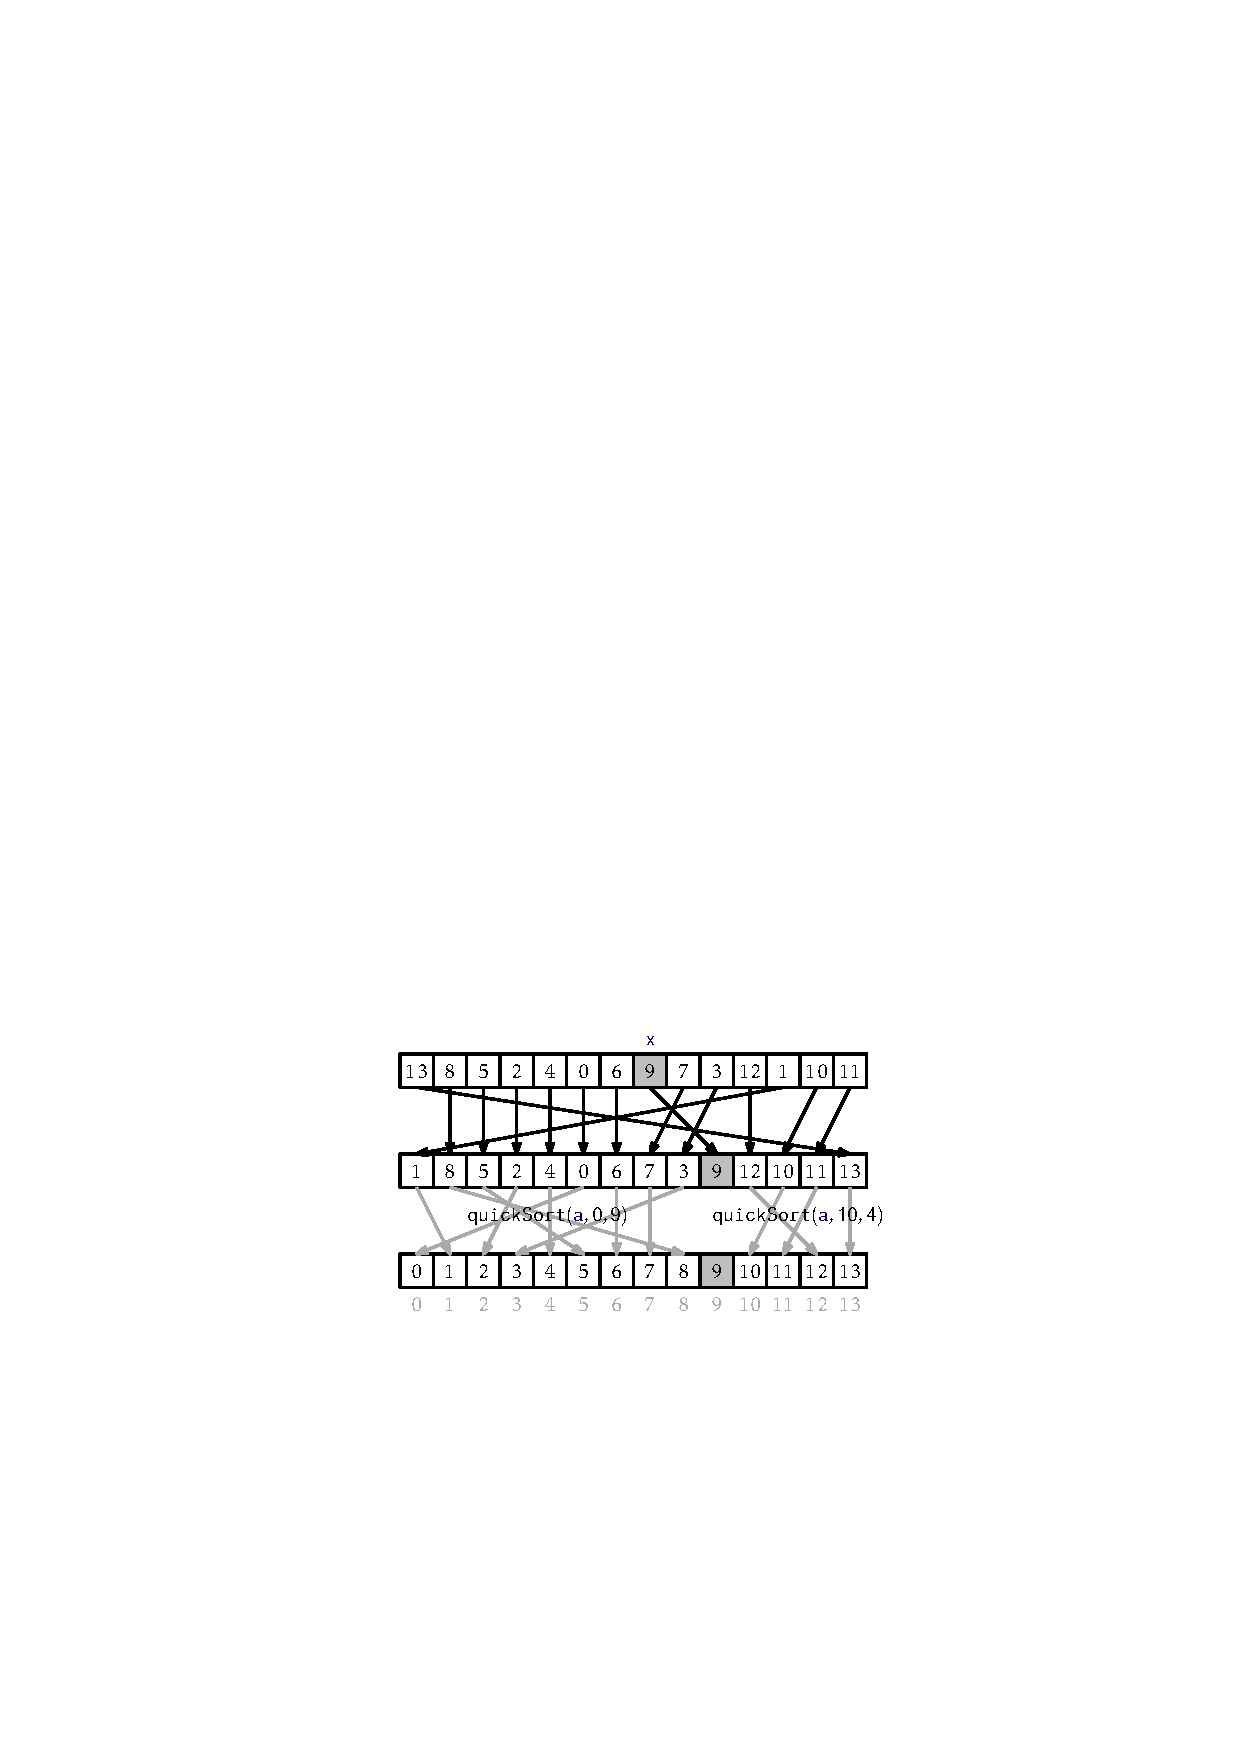
\includegraphics[scale=0.90909]{figs/quicksort}
    \caption[Quicksort]{An example execution of \javaonly{#quickSort(a,0,14,c)#}\cpponly{#quickSort(a,0,14)#}\pcodeonly{#quickSort(a,0,14)#}}
    \figlabel{quicksort}
  \end{center}
\end{figure}
All of this is done in place, so that instead of making copies of
subarrays being sorted, the #quickSort(a,i,n,c)# method only sorts the
subarray $#a[i]#,\ldots,#a[i+n-1]#$.  Initially, this method is invoked
with the arguments
#quickSort(a,0,a.length,c)#.

At the heart of the quicksort algorithm is the in-place partitioning
algorithm.  This algorithm, without using any extra space, swaps elements
in #a# and computes indices #p# and #q# so that
\[
   #a[i]# \begin{cases} 
         {}< #x# & \text{if $0\le #i#\le #p#$} \\
         {}= #x# & \text{if $#p#< #i# < #q#$} \\
         {}> #x# & \text{if $#q#\le #i# \le #n#-1$}
     \end{cases}
\]
This partitioning, which is done by the #while# loop in the code, works
by iteratively increasing #p# and decreasing #q# while maintaining the
first and last of these conditions.  At each step, the element at position
#j# is either moved to the front, left where it is, or moved to the back.
In the first two cases, #j# is incremented, while in the last case, #j#
is not incremented since the new element at position #j# has not yet been
processed.

Quicksort is very closely related to the random binary search trees
studied in \secref{rbst}.  In fact, if the input to quicksort consists
of #n# distinct elements, then the quicksort recursion tree is a random
binary search tree.  To see this, recall that when constructing a random
binary search tree the first thing we do is pick a random element #x# and
make it the root of the tree.  After this, every element will eventually
be compared to #x#, with smaller elements going into the left subtree
and larger elements into the right.

In quicksort, we select a random element #x# and immediately compare
everything to #x#, putting the smaller elements at the beginning of
the array and larger elements at the end of the array.  Quicksort then
recursively sorts the beginning of the array and the end of the array,
while the random binary search tree recursively inserts smaller elements
in the left subtree of the root and larger elements in the right subtree
of the root.

The above correspondence between random binary search trees and quicksort
means that we can translate \lemref{rbs} to a statement about quicksort:

\begin{lem}\lemlabel{quicksort}
  When quicksort is called to sort an array containing the integers
  $0,\ldots,#n#-1$, the expected number of times element #i# is compared
  to a pivot element is at most $H_{#i#+1} + H_{#n#-#i#}$.
\end{lem}

A little summing up of harmonic numbers gives us the following theorem
about the running time of quicksort:

\begin{thm}\thmlabel{quicksort-i}
  When quicksort is called to sort an array containing #n# distinct
  elements, the expected number of comparisons performed is at most
  $2#n#\ln #n# + O(#n#)$.
\end{thm}

\begin{proof}
Let $T$ be the number of comparisons performed by quicksort when sorting
#n# distinct elements.  Using \lemref{quicksort} and linearity of
expectation, we have:
\begin{align*}
  \E[T] &= \sum_{i=0}^{#n#-1}(H_{#i#+1}+H_{#n#-#i#}) \\ 
        &= 2\sum_{i=1}^{#n#}H_i \\ 
        &\le 2\sum_{i=1}^{#n#}H_{#n#} \\ 
        &\le 2#n#\ln#n# + 2#n# = 2#n#\ln #n# + O(#n#) \qedhere
\end{align*}
\end{proof}

\thmref{quicksort} describes the case where the elements being sorted are
all distinct.  When the input array, #a#, contains duplicate elements,
the expected running time of quicksort is no worse, and can be even
better; any time a duplicate element #x# is chosen as a pivot, all
occurrences of #x# get grouped together and do not take part in either
of the two subproblems.

\begin{thm}\thmlabel{quicksort}
  The \javaonly{#quickSort(a,c)#} \cpponly{#quickSort(a)#}
  \pcodeonly{#quickSort(a,c)#} method runs in $O(#n#\log #n#)$ expected
  time and the expected number of comparisons it performs is at most
  $2#n#\ln #n# +O(#n#)$.
\end{thm}

\subsection{Heap-sort}
\seclabel{heapsort}

\index{heap-sort}%
The \emph{heap-sort} algorithm is another in-place sorting algorithm.
Heap-sort uses the binary heaps discussed in \secref{binaryheap}.
Recall that the #BinaryHeap# data structure represents a heap using
a single array.  The heap-sort algorithm converts the input array #a#
into a heap and then repeatedly extracts the minimum value.

More specifically, a heap stores #n# elements in an array, #a#, at array locations
$#a[0]#,\ldots,#a[n-1]#$ with the smallest value stored at the root,
#a[0]#.  After transforming #a# into a #BinaryHeap#, the heap-sort
algorithm repeatedly swaps #a[0]# and #a[n-1]#, decrements #n#, and
calls #trickleDown(0)# so that $#a[0]#,\ldots,#a[n-2]#$ once again are
a valid heap representation. When this process ends (because $#n#=0$)
the elements of #a# are stored in decreasing order, so #a# is reversed
to obtain the final sorted order.\footnote{The algorithm
could alternatively redefine the #compare(x,y)# function so that the
heap sort algorithm stores the elements directly in ascending order.}
\figref{heapsort} shows an example of the execution of #heapSort(a,c)#.

\begin{figure}
  \begin{center}
    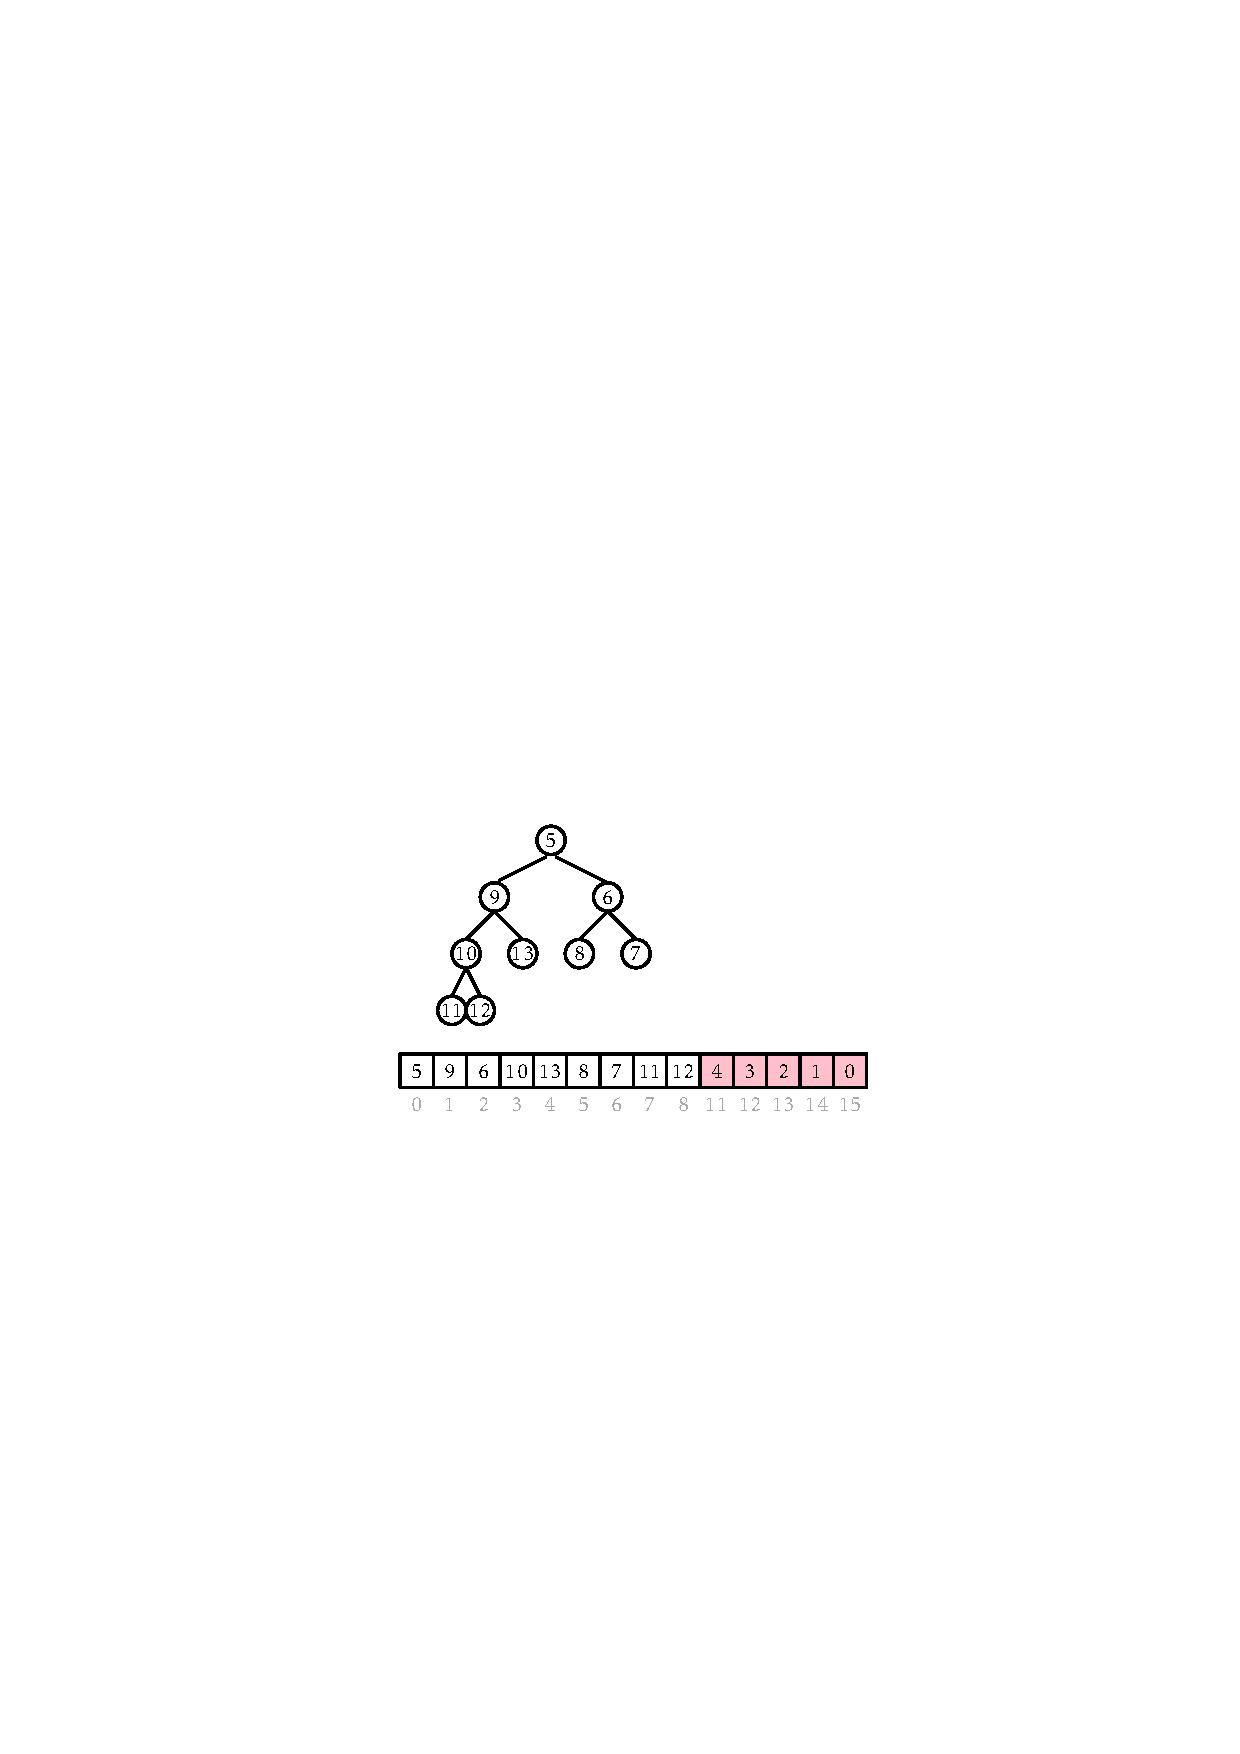
\includegraphics[scale=0.90909]{figs/heapsort}
  \end{center}
  \caption[Heap sort]{A snapshot of the execution of #heapSort(a,c)#.
      The shaded part of the
      array is already sorted.  The unshaded part is a #BinaryHeap#.
      During the next iteration, element $5$ will be placed into array
      location $8$.}
  \figlabel{heapsort}
\end{figure}

\javaimport{ods/BinaryHeap.sort(a,c)}
\cppimport{ods/BinaryHeap.sort(b)}
\pcodeimport{ods/Algorithms.heapSort(a)}

A key subroutine in heap sort is the constructor for turning
an unsorted array #a# into a heap.  It would be easy to do this
in $O(#n#\log#n#)$ time by repeatedly calling the #BinaryHeap#
#add(x)# method, but we can do better by using a bottom-up algorithm.
Recall that, in a binary heap, the children of #a[i]# are stored at
positions #a[2i+1]# and #a[2i+2]#.  This implies that the elements
$#a#[\lfloor#n#/2\rfloor],\ldots,#a[n-1]#$ have no children. In other
words, each of $#a#[\lfloor#n#/2\rfloor],\ldots,#a[n-1]#$ is a sub-heap
of size 1.  Now, working backwards, we can call #trickleDown(i)# for
each $#i#\in\{\lfloor #n#/2\rfloor-1,\ldots,0\}$. This works, because by
the time we call #trickleDown(i)#, each of the two children of #a[i]#
are the root of a sub-heap, so calling #trickleDown(i)# makes #a[i]#
into the root of its own subheap.
\javaimport{ods/BinaryHeap.BinaryHeap(a,c)}
\cppimport{ods/BinaryHeap.BinaryHeap(b)}

The interesting thing about this bottom-up strategy is that it is more
efficient than calling #add(x)# #n# times.  To see this, notice that,
for $#n#/2$ elements, we do no work at all, for $#n#/4$ elements, we call
#trickleDown(i)# on a subheap rooted at #a[i]# and whose height is one, for
$#n#/8$ elements, we call #trickleDown(i)# on a subheap whose height is two,
and so on.  Since the work done by #trickleDown(i)# is proportional to
the height of the sub-heap rooted at #a[i]#, this means that the total
work done is at most
\[
    \sum_{i=1}^{\log#n#} O((i-1)#n#/2^{i})
    \le \sum_{i=1}^{\infty} O(i#n#/2^{i})
    = O(#n#)\sum_{i=1}^{\infty} i/2^{i}
    =  O(2#n#) = O(#n#) \enspace .
\]
The second-last equality follows by recognizing that the sum
$\sum_{i=1}^{\infty} i/2^{i}$ is equal, by definition of expected value,
to the expected number of times we toss a coin up to and including the
first time the coin comes up as heads and applying \lemref{coin-tosses}.

The following theorem describes the performance of #heapSort(a,c)#.
\begin{thm}
  The #heapSort(a,c)# method runs in $O(#n#\log #n#)$ time and performs at
  most $2#n#\log #n# + O(#n#)$ comparisons.
\end{thm}

\begin{proof}
The algorithm runs in three steps:  (1)~transforming #a# into a heap,
(2)~repeatedly extracting the minimum element from #a#, and (3)~reversing
the elements in #a#.  We have just argued that step~1 takes $O(#n#)$
time and performs $O(#n#)$ comparisons.  Step~3 takes $O(#n#)$ time and
performs no comparisons.  Step~2 performs #n# calls to #trickleDown(0)#.
The $i$th such call operates on a heap of size $#n#-i$ and performs
at most $2\log(#n#-i)$ comparisons.  Summing this over $i$ gives
\[
   \sum_{i=0}^{#n#-i} 2\log(#n#-i) 
   \le \sum_{i=0}^{#n#-i} 2\log #n#
   =  2#n#\log #n#
\]
Adding the number of comparisons performed in each of the three steps
completes the proof.
\end{proof}

\subsection{A Lower-Bound for Comparison-Based Sorting}

\index{lower-bound}%
\index{sorting lower-bound}%
We have now seen three comparison-based sorting algorithms that each run
in $O(#n#\log #n#)$ time.  By now, we should be wondering if faster
algorithms exist.  The short answer to this question is no.  If the
only operations allowed on the elements of #a# are comparisons, then no
algorithm can avoid doing roughly $#n#\log #n#$ comparisons.  This is
not difficult to prove, but requires a little imagination.  Ultimately,
it follows from the fact that
\[
   \log(#n#!) 
     = \log #n# + \log (#n#-1) + \dots + \log(1) 
     = #n#\log #n# - O(#n#)
    \enspace .
\]
(Proving this fact is left as \excref{log-factorial}.)

We will start by focusing our attention on deterministic algorithms like
merge-sort and heap-sort and on a particular fixed value of #n#.  Imagine
such an algorithm is being used to sort #n# distinct elements.  The key
to proving the lower-bound is to observe that, for a deterministic
algorithm with a fixed value of #n#, the first pair of elements that are
compared is always the same.  For example, in #heapSort(a,c)#, when #n#
is even, the first call to #trickleDown(i)# is with #i=n/2-1# and the
first comparison is between elements #a[n/2-1]# and #a[n-1]#.

Since all input elements are distinct, this first comparison has only
two possible outcomes.  The second comparison done by the algorithm may
depend on the outcome of the first comparison.  The third comparison
may depend on the results of the first two, and so on.  In this way,
any deterministic comparison-based sorting algorithm can be viewed
as a rooted binary \emph{comparison tree}.
\index{comparison tree}%
Each internal node, #u#,
of this tree is labelled with a pair of indices #u.i# and #u.j#.
If $#a[u.i]#<#a[u.j]#$ the algorithm proceeds to the left subtree,
otherwise it proceeds to the right subtree.  Each leaf #w# of this
tree is labelled with a permutation $#w.p[0]#,\ldots,#w.p[n-1]#$ of
$0,\ldots,#n#-1$.  This permutation represents the one that is
required to sort #a# if the comparison tree reaches this leaf.  That is,
\[
   #a[w.p[0]]#<#a[w.p[1]]#<\cdots<#a[w.p[n-1]]# \enspace .
\]
An example of a comparison tree for an array of size #n=3# is shown in
\figref{comparison-tree}.
\begin{figure}
  \begin{center}
    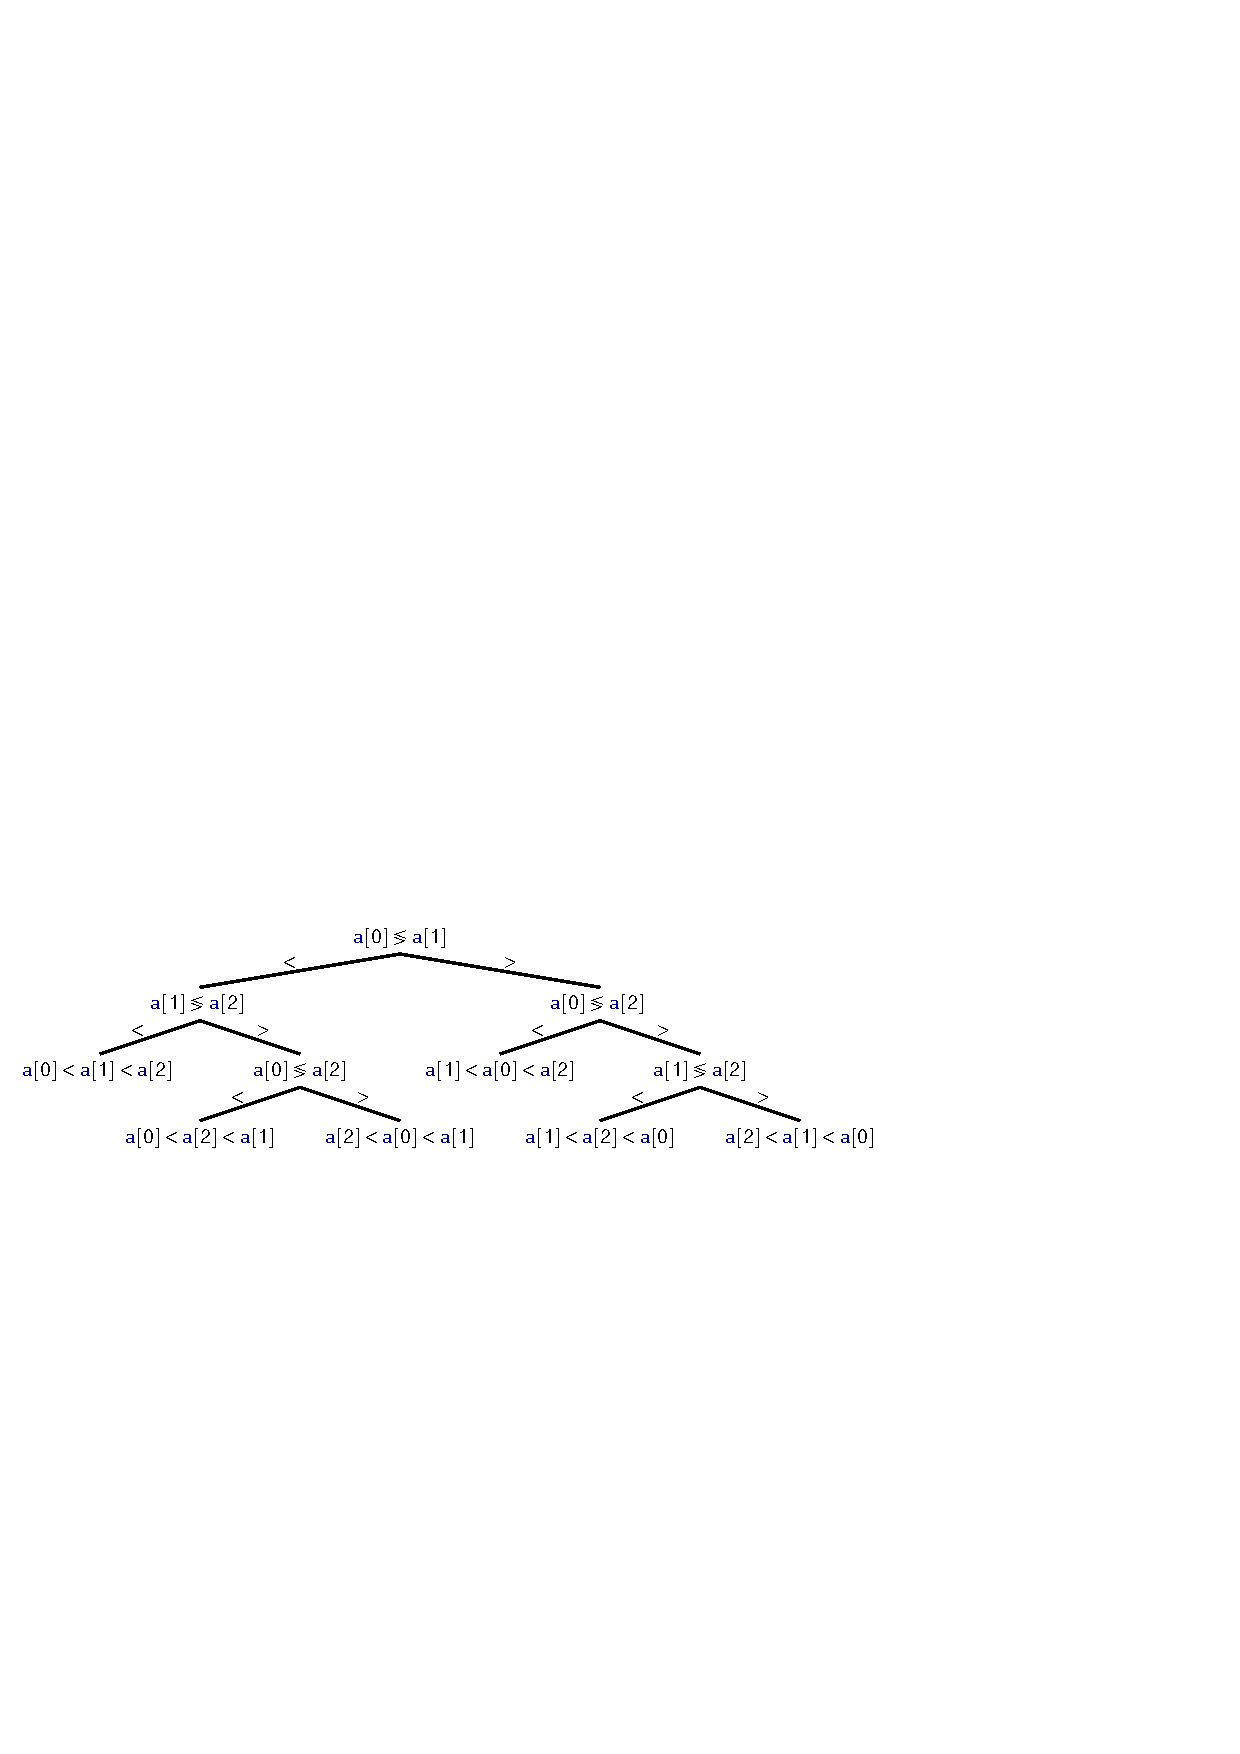
\includegraphics[width=\ScaleIfNeeded]{figs/comparison-tree}
  \end{center}
  \caption[A comparison tree]{A comparison tree for sorting an array $#a[0]#,#a[1]#,#a[2]#$ of length #n=3#.}
  \figlabel{comparison-tree}
\end{figure}

The comparison tree for a sorting algorithm tells us everything about
the algorithm.  It tells us exactly the sequence of comparisons that
will be performed for any input array, #a#, having #n# distinct elements
and it tells us how the algorithm will reorder #a# in order to sort it.
Consequently, the comparison tree must have at least $#n#!$ leaves;
if not, then there are two distinct permutations that lead to the same
leaf; therefore, the algorithm does not correctly sort at least one of
these permutations.

For example, the comparison tree in \figref{comparison-tree-2} has only
$4< 3!=6$ leaves. Inspecting this tree, we see that the two input arrays
$3,1,2$ and $3,2,1$ both lead to the rightmost leaf.  On the input $3,1,2$
this leaf correctly outputs $#a[1]#=1,#a[2]#=2,#a[0]#=3$.  However, on the
input $3,2,1$, this node incorrectly outputs $#a[1]#=2,#a[2]#=1,#a[0]#=3$.
This discussion leads to the primary lower-bound for comparison-based
algorithms.

\begin{figure}
  \begin{center}
    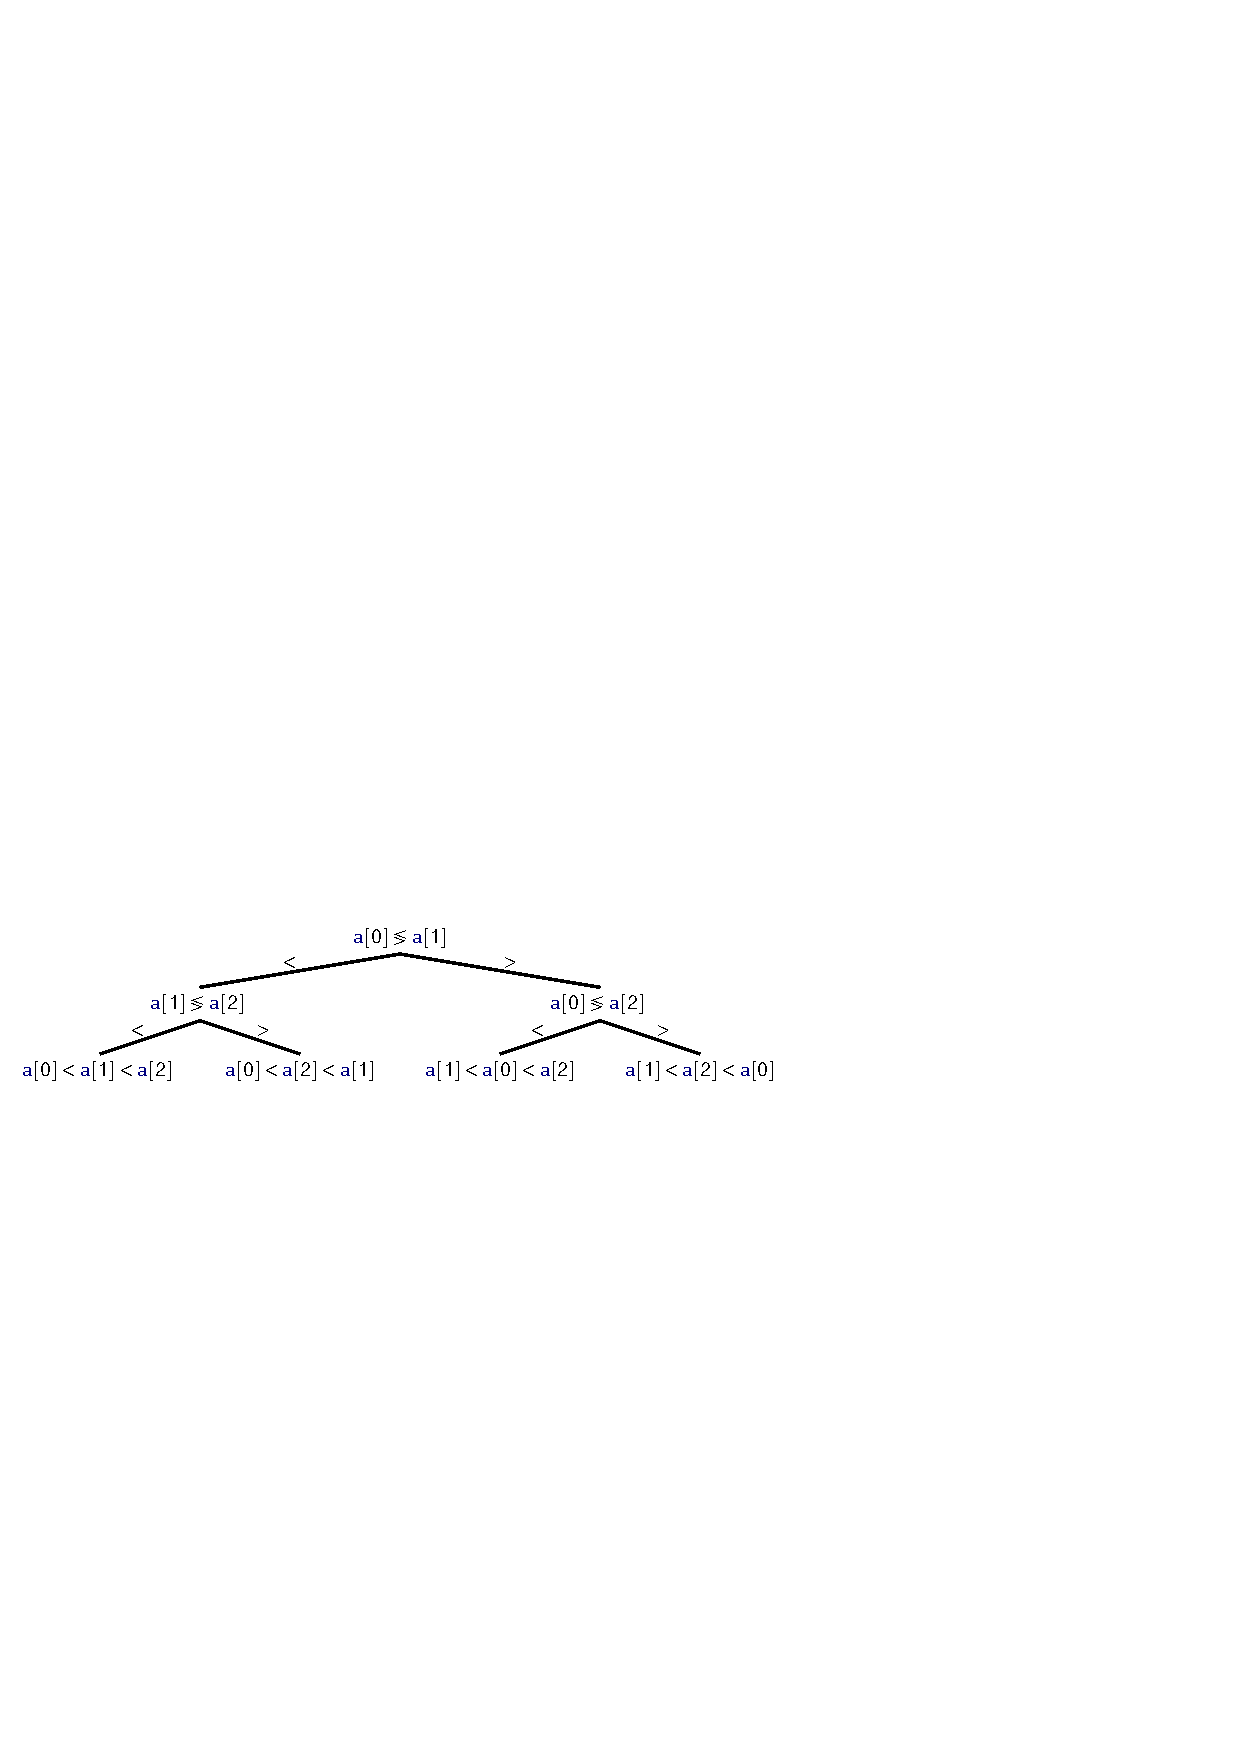
\includegraphics[width=\ScaleIfNeeded]{figs/comparison-tree-b}
  \end{center}
  \caption{A comparison tree that does not correctly sort every input
  permutation.}
  \figlabel{comparison-tree-2}
\end{figure}

\begin{thm}\thmlabel{deterministic-sorting-lower-bound}
  For any deterministic comparison-based sorting algorithm $\mathcal{A}$
  and any integer $#n#\ge 1$, there exists an input array #a# of
  length #n# such that $\mathcal{A}$ performs at least $\log(#n#!) =
  #n#\log#n#-O(#n#)$ comparisons when sorting #a#.
\end{thm}

\begin{proof}
  By the preceding discussion, the comparison tree defined by $\mathcal{A}$
  must have at least $#n#!$ leaves.  An easy inductive proof shows that
  any binary tree with $k$ leaves has a height of at least $\log k$.
  Therefore, the comparison tree for $\mathcal{A}$ has a leaf, #w#,
  with a depth of at least $\log(#n#!)$ and there is an input array #a#
  that leads to this leaf.  The input array #a# is an input for which
  $\mathcal{A}$ does at least $\log(#n#!)$ comparisons.
\end{proof}

\thmref{deterministic-sorting-lower-bound} deals with deterministic
algorithms like merge-sort and heap-sort, but doesn't tell us anything
about randomized algorithms like quicksort.  Could a randomized algorithm
beat the $\log(#n#!)$ lower bound on the number of comparisons?
The answer, again, is no.  Again, the way to prove it is to think
differently about what a randomized algorithm is.

In the following discussion, we will assume that our decision
trees have been ``cleaned up'' in the following way: Any node that can not
be reached by some input array #a# is removed.  This cleaning up implies
that the tree has exactly $#n#!$ leaves.  It has at least $#n#!$ leaves
because, otherwise, it could not sort correctly.  It has at most $#n#!$
leaves since each of the possible $#n#!$ permutation of #n# distinct
elements follows exactly one root to leaf path in the decision tree.

We can think of a randomized sorting algorithm, $\mathcal{R}$, as a
deterministic algorithm that takes two inputs: The input array #a#
that should be sorted and a long sequence $b=b_1,b_2,b_3,\ldots,b_m$
of random real numbers in the range $[0,1]$.  The random numbers provide
the randomization for the algorithm.  When the algorithm wants to toss a
coin or make a random choice, it does so by using some element from $b$.
For example, to compute the index of the first pivot in quicksort,
the algorithm could use the formula $\lfloor n b_1\rfloor$.

Now, notice that if we fix $b$ to some particular sequence $\hat{b}$
then $\mathcal{R}$ becomes a deterministic sorting algorithm,
$\mathcal{R}(\hat{b})$, that has an associated comparison tree,
$\mathcal{T}(\hat{b})$.  Next, notice that if we select #a# to be a random
permutation of $\{1,\ldots,#n#\}$, then this is equivalent to selecting
a random leaf, #w#, from the $#n#!$ leaves of $\mathcal{T}(\hat{b})$.

\excref{randomized-lower-bound} asks you to prove that, if we select
a random leaf from any binary tree with $k$ leaves, then the expected
depth of that leaf is at least $\log k$.  Therefore, the expected
number of comparisons performed by the (deterministic) algorithm
$\mathcal{R}(\hat{b})$ when given an input array containing a random
permutation of $\{1,\ldots,n\}$ is at least $\log(#n#!)$.  Finally,
notice that this is true for every choice of $\hat{b}$, therefore it holds even for $\mathcal{R}$.  This completes the proof of the lower-bound for randomized algorithms.

\begin{thm}\thmlabel{randomized-sorting-lower-bound}
  For any integer $n\ge 1$ and any  (deterministic or randomized)
  comparison-based sorting algorithm $\mathcal{A}$, the expected number
  of comparisons done by $\mathcal{A}$ when sorting a random permutation
  of $\{1,\ldots,n\}$ is at least $\log(#n#!) = #n#\log#n#-O(#n#)$.
\end{thm}



\section{Counting Sort and Radix Sort}

In this section we study two sorting algorithms that are not
comparison-based. Specialized for sorting small integers, these algorithms
elude the lower-bounds of \thmref{deterministic-sorting-lower-bound}
by using (parts of) the elements in #a# as indices into an array.
Consider a statement of the form
\[
  #c[a[i]]# = 1 \enspace .
\]
This statement executes in constant time, but has #c.length# possible
different outcomes, depending on the value of #a[i]#.  This means that the
execution of an algorithm that makes such a statement cannot be modelled
as a binary tree.  Ultimately, this is the reason that the algorithms
in this section are able to sort faster than comparison-based algorithms.

\subsection{Counting Sort}

Suppose we have an input array #a# consisting of #n# integers, each in
the range $0,\ldots,#k#-1$.  The \emph{counting-sort}
\index{counting-sort}%
algorithm sorts #a#
using an auxiliary array #c# of counters.  It outputs a sorted version
of #a# as an auxiliary array #b#.

The idea behind counting-sort is simple:  For each
$#i#\in\{0,\ldots,#k#-1\}$, count the number of occurrences of #i# in #a#
and store this in #c[i]#.  Now, after sorting, the output will look like
#c[0]# occurrences of 0, followed by #c[1]# occurrences of 1, followed by
#c[2]# occurrences of 2,\ldots, followed by #c[k-1]# occurrences of #k-1#.
The code that does this is very slick, and its execution is illustrated in
\figref{countingsort}:
\codeimport{ods/Algorithms.countingSort(a,k)}

\begin{figure}
  \begin{center}
    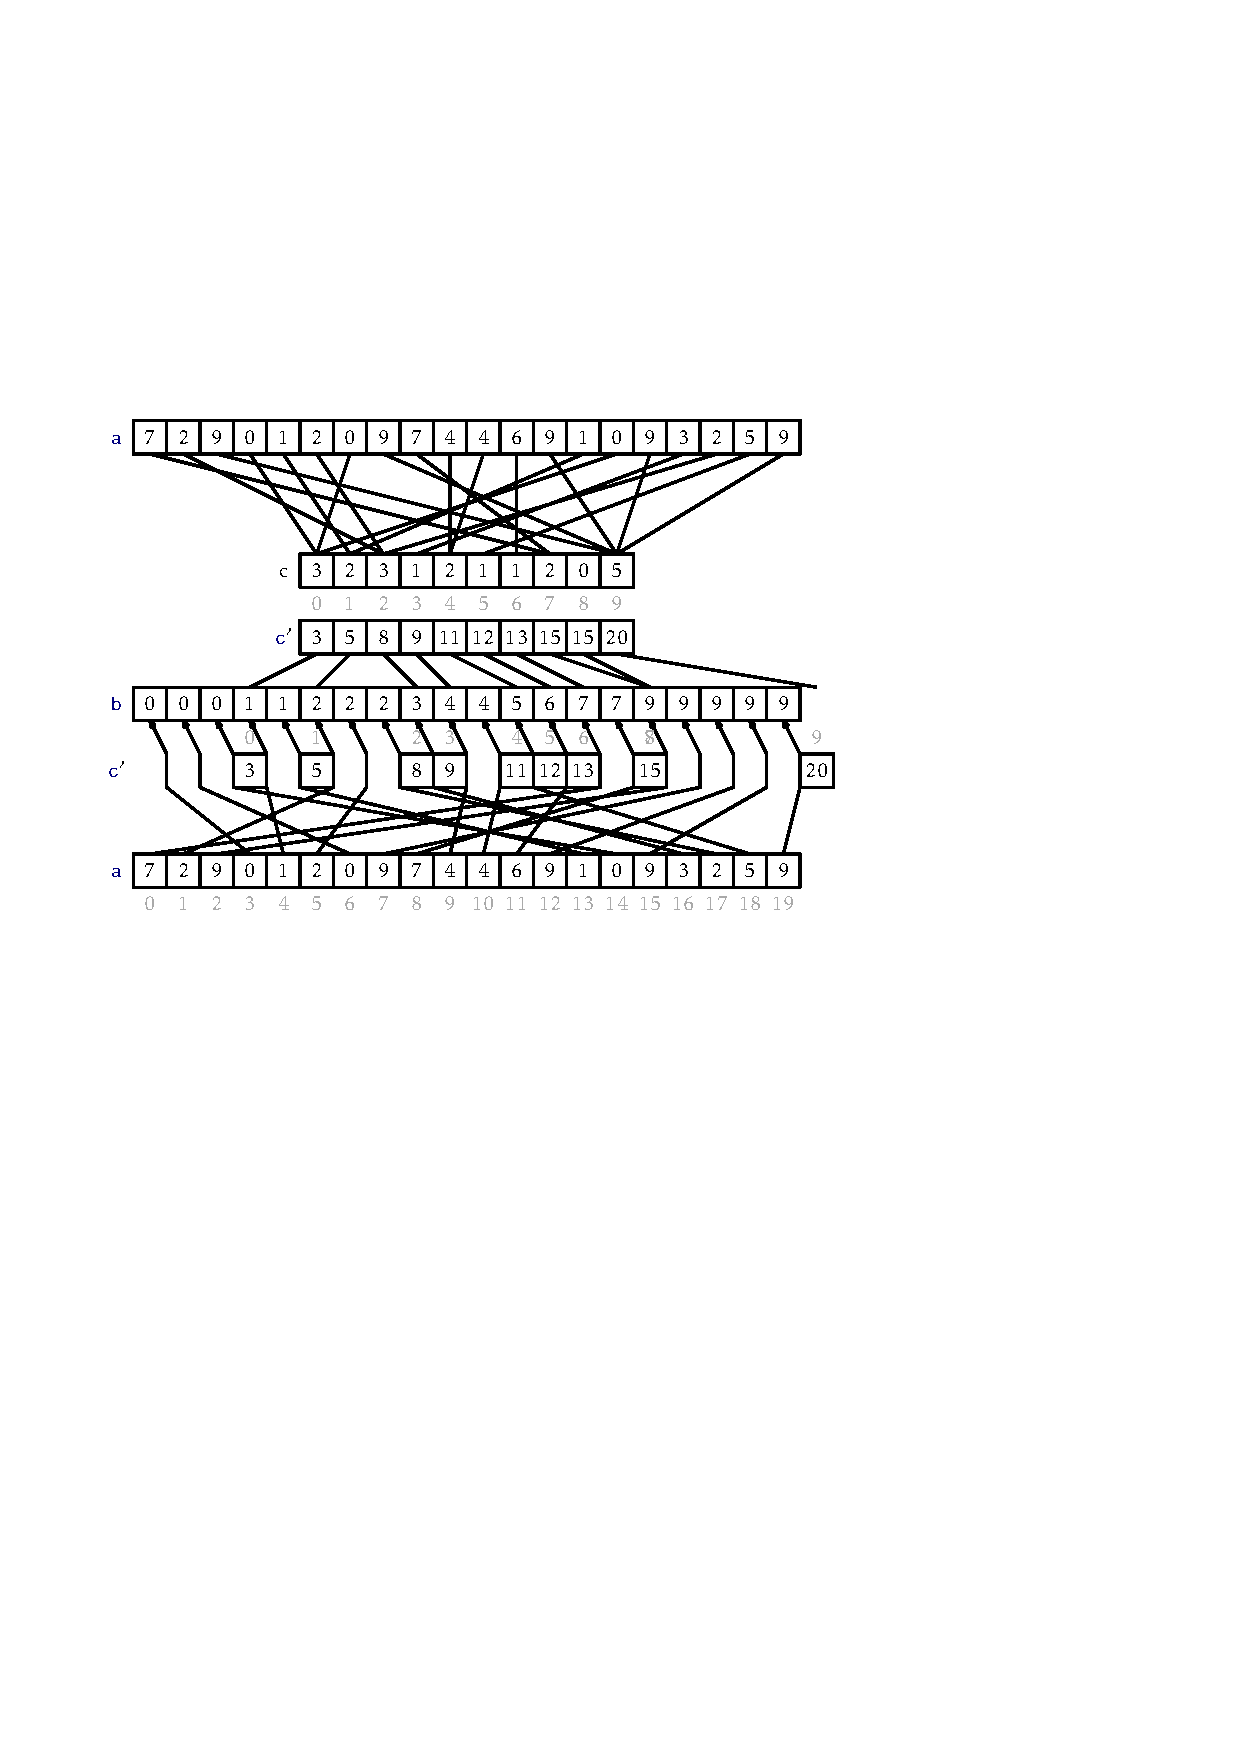
\includegraphics[width=\ScaleIfNeeded]{figs/countingsort}
  \end{center}
  \caption{The operation of counting sort on an array of length $#n#=20$ that stores integers $0,\ldots,#k#-1=9$.}
  \figlabel{countingsort}
\end{figure}

The first #for# loop in this code sets each counter #c[i]# so that it
counts the number of occurrences of #i# in #a#.  By using the values
of #a# as indices, these counters can all be computed in $O(#n#)$ time
with a single for loop.  At this point, we could use #c# to
fill in the output array #b# directly. However, this would not work if
the elements of #a# have associated data.  Therefore we spend a little
extra effort to copy the elements of #a# into #b#.

The next #for# loop, which takes $O(#k#)$ time, computes a running-sum
of the counters so that #c[i]# becomes the number of elements in
#a# that are less than or equal to #i#.  In particular, for every
$#i#\in\{0,\ldots,#k#-1\}$, the output array, #b#, will have
\[
   #b[c[i-1]]#=#b[c[i-1]+1]=#\cdots=#b[c[i]-1]#=#i# \enspace .
\]
Finally, the algorithm scans #a# backwards to place its elements, in order,
into an output array #b#.  When scanning, the element #a[i]=j# is placed
at location #b[c[j]-1]# and the value #c[j]# is decremented.

\begin{thm}
  The #countingSort(a,k)# method can sort an array #a# containing #n#
  integers in the set $\{0,\ldots,#k#-1\}$ in $O(#n#+#k#)$ time.
\end{thm}

The counting-sort algorithm has the nice property of being \emph{stable};
\index{stable sorting algorithm}%
it preserves the relative order of equal elements.  If two elements
#a[i]# and #a[j]# have the same value, and $#i#<#j#$ then #a[i]# will
appear before #a[j]# in #b#.  This will be useful in the next section.

\subsection{Radix-Sort}

Counting-sort is very efficient for sorting an array of integers when the
length, #n#, of the array is not much smaller than the maximum value,
$#k#-1$, that appears in the array.  The \emph{radix-sort}
\index{radix-sort}%
algorithm,
which we now describe, uses several passes of counting-sort to allow
for a much greater range of maximum values.

Radix-sort sorts #w#-bit integers by using $#w#/#d#$ passes of counting-sort
to sort these integers #d# bits at a time.\footnote{We assume that
#d# divides #w#, otherwise we can always increase #w# to $#d#\lceil
#w#/#d#\rceil$.}  More precisely, radix sort first sorts the integers by
their least significant #d# bits, then their next significant #d# bits,
and so on until, in the last pass, the integers are sorted by their most
significant #d# bits.
\codeimport{ods/Algorithms.radixSort(a)}
(In this code, the expression #(a[i]>>d*p)&((1<<d)-1)# extracts the integer
whose binary representation is given by bits
$(#p#+1)#d#-1,\ldots,#p##d#$ of #a[i]#.)
An example of the steps of this algorithm is shown in \figref{radixsort}.

\begin{figure}
  \begin{center}
    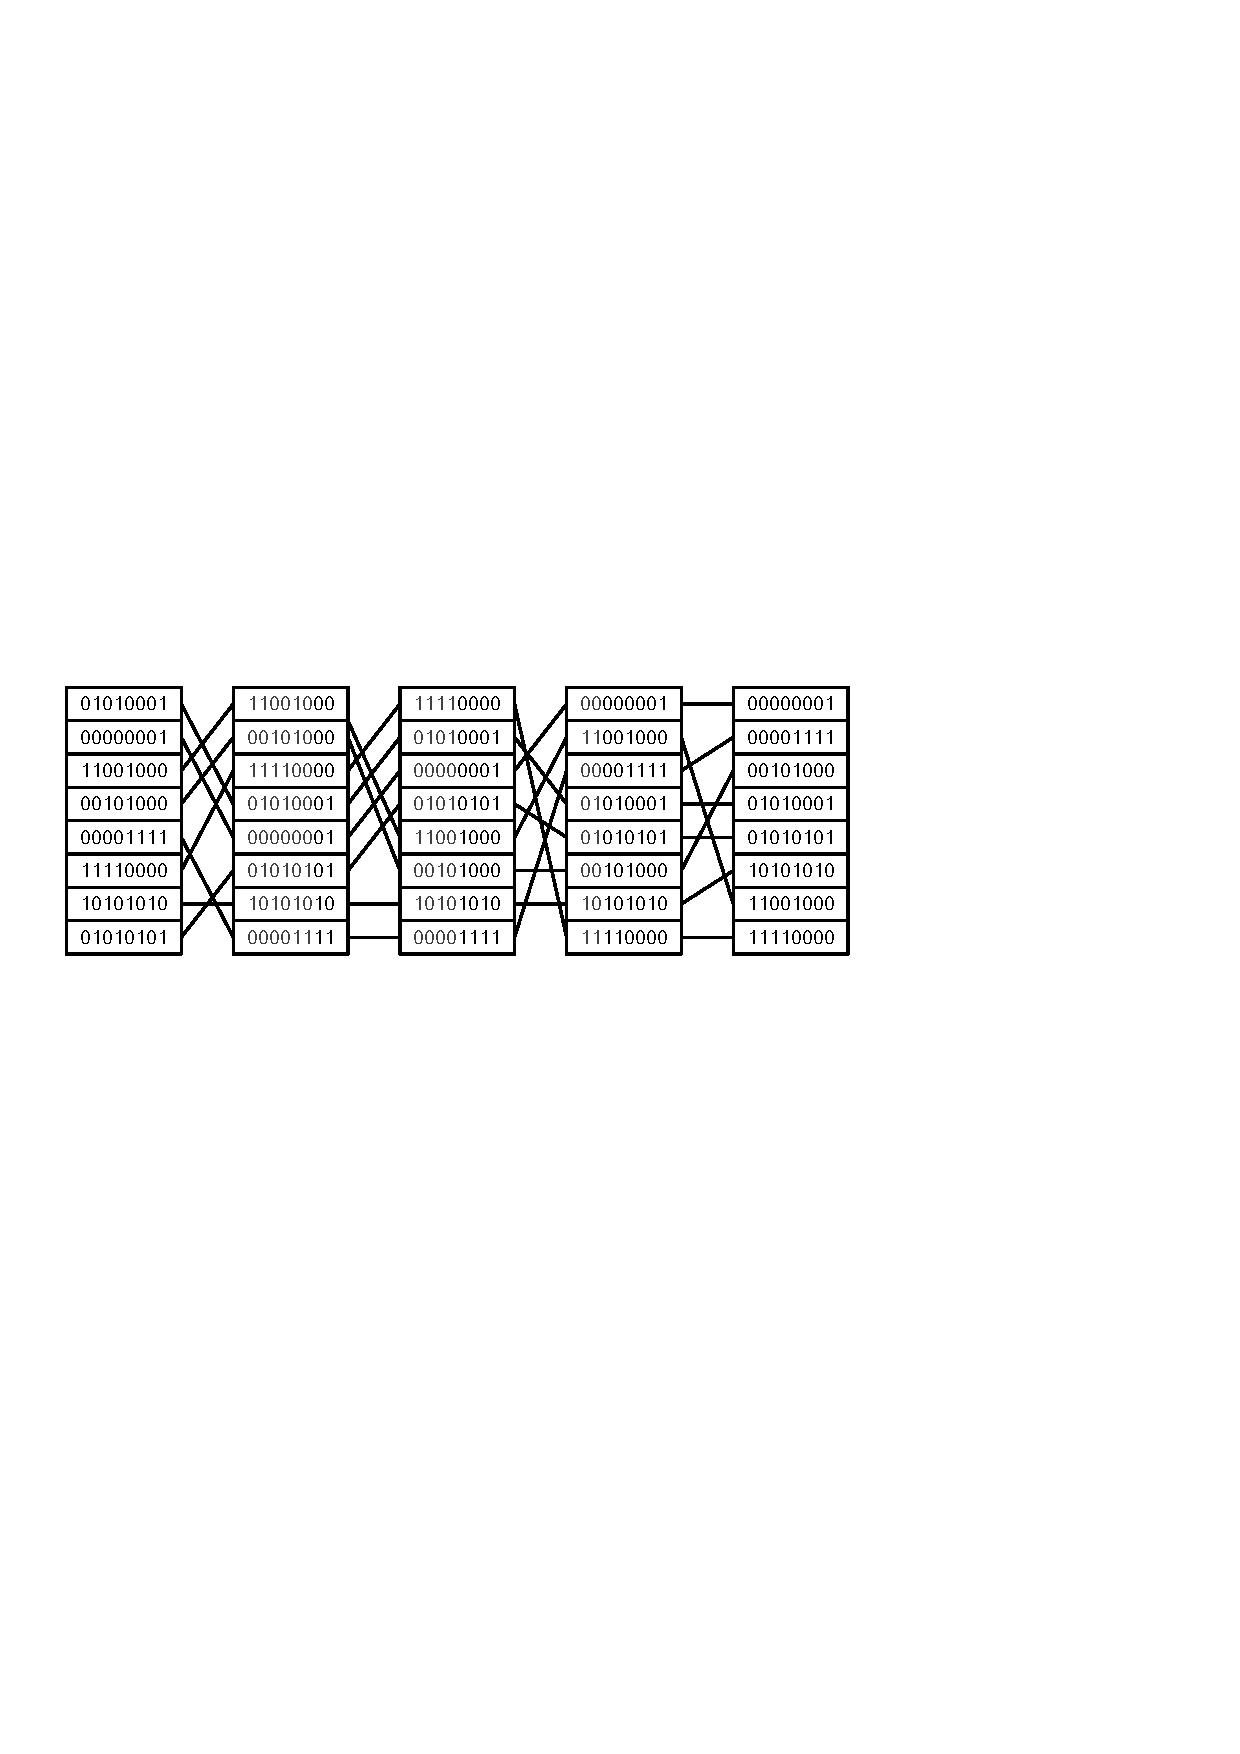
\includegraphics[width=\ScaleIfNeeded]{figs/radixsort}
  \end{center}
  \caption{Using radixsort to sort $#w#=8$-bit integers by using 4 passes
   of counting sort on $#d#=2$-bit integers.}
  \figlabel{radixsort}
\end{figure}

This remarkable algorithm sorts correctly because counting-sort is
a stable sorting algorithm.  If $#x# < #y#$ are two elements of #a#,
and the most significant bit at which #x# differs from #y# has index $r$,
then #x# will be placed before #y# during pass $\lfloor r/#d#\rfloor$
and subsequent passes will not change the relative order of #x# and #y#.

Radix-sort performs #w/d# passes of counting-sort.  Each pass requires
$O(#n#+2^{#d#})$ time. Therefore, the performance of radix-sort is given
by the following theorem.
\begin{thm}\thmlabel{radix-sort}
  For any integer $#d#>0$, the #radixSort(a,k)# method can sort an array
  #a# containing #n# #w#-bit integers in $O((#w#/#d#)(#n#+2^{#d#}))$ time.
\end{thm}

If we think, instead, of the elements of the array being in the range
$\{0,\ldots,#n#^c-1\}$, and take $#d#=\lceil\log#n#\rceil$ we obtain
the following version of \thmref{radix-sort}.
\begin{cor}\corlabel{radix-sort-poly}
  The #radixSort(a,k)# method can sort an array #a# containing #n#
  integer values in the range $\{0,\ldots,#n#^c-1\}$ in $O(c#n#)$ time.
\end{cor}

\section{Discussion and Exercises}

Sorting is \emph{the} fundamental algorithmic problem in computer science,
and it has a long history.  Knuth \cite{k97v3} attributes the merge-sort
algorithm to von~Neumann (1945).  Quicksort is due to Hoare \cite{h61}.
The original heap-sort algorithm is due to Williams \cite{w64}, but the
version presented here (in which the heap is constructed bottom-up
in $O(#n#)$ time) is due to Floyd \cite{f64}.  Lower-bounds for
comparison-based sorting appear to be folklore.  The following table
summarizes the performance of these comparison-based algorithms:

\begin{center}
  \begin{tabular}{|l|r@{}l@{ }l|l|} \hline
      & \multicolumn{3}{c|}{comparisons} & in-place  \\ \hline
    Merge-sort & $#n#\log #n#$ & &  worst-case & No  \\
    Quicksort & $1.38#n#\log #n#$ & ${}+ O(#n#)$ & expected & Yes \\
    Heap-sort & $2#n#\log #n#$ & ${}+ O(#n#)$ & worst-case & Yes \\ \hline
  \end{tabular}
\end{center}

Each of these comparison-based algorithms has its advantages and
disadvantages.  Merge-sort does the fewest comparisons and does not rely
on randomization.  Unfortunately, it uses an auxilliary array during its
merge phase.  Allocating this array can be expensive and is a potential
point of failure if memory is limited.  Quicksort is an \emph{in-place}
\index{in-place algorithm}%
algorithm and is a close second in terms of the number of comparisons,
but is randomized, so this running time is not always guaranteed.
Heap-sort does the most comparisons, but it is in-place and deterministic.

There is one setting in which merge-sort is a clear-winner;  this
occurs when sorting a linked-list.  In this case, the auxiliary
array is not needed;  two sorted linked lists are very easily merged
into a single sorted linked-list by pointer manipulations (see
\excref{list-merge-sort}).

The counting-sort and radix-sort algorithms described here are due
to Seward \cite[Section~2.4.6]{s54}.  However, variants of radix-sort
have been used since the 1920s to sort punch cards using punched card
sorting machines.  These machines can sort a stack of cards into two
piles based on the existence (or not) of a hole in a specific location
on the card.  Repeating this process for different hole locations gives
an implementation of radix-sort.

Finally, we note that counting sort and radix-sort can be used to sort
other types of numbers besides non-negative integers.  Straightforward
modifications of counting sort can sort integers, in any interval
$\{a,\ldots,b\}$, in $O(#n#+b-a)$ time.  Similarly, radix sort can sort
integers in the same interval in $O(#n#(\log_{#n#}(b-a))$ time.  Finally, both of these
algorithms can also be used to sort floating point numbers in the IEEE 754
floating point format.  This is because the IEEE format is designed to
allow the comparison of two floating point numbers by comparing their values
as if they were integers in a signed-magnitude binary representation
\cite{ieee754}.

\begin{exc}
  Illustrate the execution of merge-sort and heap-sort on an input array
  containing $1,7,4,6,2,8,3,5$.  Give a sample illustration of one possible
  execution of quicksort on the same array.
\end{exc}

\begin{exc}\exclabel{list-merge-sort}
  Implement a version of the merge-sort algorithm that sorts a #DLList#
  without using an auxiliary array. (See \excref{dllist-sort}.) 
\end{exc}

\begin{exc}
  Some implementations of #quickSort(a,i,n,c)# always use #a[i]#
  as a pivot.  Give an example of an input array of length #n# in which
  such an implementation would perform $\binom{#n#}{2}$ comparisons.
\end{exc}

\begin{exc}
  Some implementations of #quickSort(a,i,n,c)# always use #a[i+n/2]#
  as a pivot.  Given an example of an input array of length #n# in which
  such an implementation would perform $\binom{#n#}{2}$ comparisons.
\end{exc}

\begin{exc}
  Show that, for any implementation of #quickSort(a,i,n,c)#
  that chooses a pivot deterministically, without first looking at
  any values in $#a[i]#,\ldots,#a[i+n-1]#$, there exists an input array of length #n#
  that causes this implementation to perform $\binom{#n#}{2}$ comparisons.
\end{exc}

\begin{exc}
  Design a #Comparator#, #c#, that you could pass as an argument
  to #quickSort(a,i,n,c)# and that would cause quicksort to perform
  $\binom{#n#}{2}$ comparisons.  (Hint: Your comparator does not actually
  need to look at the values being compared.)
\end{exc}

\begin{exc}
  Analyze the expected number of comparisons done by Quicksort a little
  more carefully than the proof of \thmref{quicksort}.  In particular, show
  that the expected number of comparisons is $2#n#H_#n# -#n# + H_#n#$.
\end{exc}

\begin{exc}
  Describe an input array that causes heap sort to perform at least
  $2#n#\log #n#-O(#n#)$ comparisons.  Justify your answer.
\end{exc}

\javaonly{
\begin{exc}
  The heap sort implementation described here sorts the elements into
  reverse sorted order and then reverses the array.  This last step
  could be avoided by defining a new #Comparator# that negates the
  results of the input #Comparator#, #c#.  Explain why this would not
  be a good optimization.  (Hint: Consider how many negations would need
  to be done in relation to how long it takes to reverse the array.)
\end{exc}
}

\begin{exc}
  Find another pair of permutations of $1,2,3$ that are not correctly
  sorted by the comparison tree in \figref{comparison-tree-2}.
\end{exc}

\begin{exc}\exclabel{log-factorial}
  Prove that $\log #n#! = #n#\log #n#-O(#n#)$.
\end{exc}

\begin{exc}
  Prove that a binary tree with $k$ leaves has height at least $\log k$.
\end{exc}

\begin{exc}\exclabel{randomized-lower-bound}
  Prove that, if we pick a random leaf from a binary tree with $k$
  leaves, then the expected height of this leaf is at least $\log k$.
%  (Hint: Use induction along with the inequality $(k_1/k)\log k_1 +
%  (k_2/k)\log k_2) \ge  \log k-1$, when $k_1+k_2=k$.)
\end{exc}

% This was a stupid exercise, since IEEE 754 floating point numbers 
% are correctly ordered when they are treated as signed magnitude integers
% [i.e., a sign bit followed by an integer ]
%\begin{exc}
%  Simple floating point numbers are numbers of the form $x\cdot10^{y}$,
%  where $0\le x\le 1$ and $y$ is an integer and each of $x$ and $y$ can
%  be represented by at most $k$ bits.  Describe a version of radix-sort
%  that can be used to sort simple floating point numbers.
%
%  Extend your version of radix sort so that it can handle signed values
%  of both $x$ and $y$ and implement a version of radix-sort that sorts
%  arrays of type #float#.
%\end{exc}

\begin{exc}
  The implementation of #radixSort(a,k)# given here works when the input
  array, #a# contains only \cpponly{unsigned}\javaonly{non-negative}
  integers.  \javaonly{Extend this implementation so that it also
  works correctly when #a# contains both negative and non-negative
  integers.}\cpponly{Write a version that works correctly for signed
  integers.}
\end{exc}

